\begin{question}
	Wat is een orakelmachine? Bespreek de uitspraak "de verzameling orakelmachines (over een gegeven orakel) is strikt krachtiger dan de verzameling van Turing machines". Leg hierbij ook uit wat men bedoeld met "krachtiger". Kan een verzameling orakelmachines (voor bepaald gegeven orakel) alle talen beslissen? Kan een orakelmachine ook $A_{TM}$ of $H_{TM}$ beslissen?
\end{question}

\subsubsection*{Orakelmachine}

Zoals we weten is een Turingmachine een handig hulpmiddel om te bepalen of strings tot een taal horen of niet. We kunnen de machines gebruiken om talen te herkennen, of specifieker, te beslissen. Niet alle talen kunnen echter beslist worden door zo een Turingmachine. Zo is het bijvoorbeeld onmogelijk om een Turingmachine op te stellen die de taal $A_{TM}$ beslist.
\\\\
Dit zorgt er voor dat we op zoek moeten gaan naar een betere machine die naast het beslissen van de al besliste talen, ook andere talen kan beslissen. De nieuwe machine moet dus krachtiger zijn. Het resultaat is een orakelmachine.
\\\\
Een orakelmachine is een uitbreiding op de Turingmachine, die een orakel bevat. Je kan een orakel bekijken als een black box waar de Turingmachine vragen een kan stellen. In theorie is een orakel eigenlijk een soort bitmap, of anders gezegd een rij van booleans. Stel we ordenen alle strings volgens de lexicografische orde met kortere strings eerst. Elke string op index $i$ komt nu overeen met een booleaanse waarde in de bitmap, die ook gealloceerd is op locatie $i$. Indien de string op een bepaalde locatie tot een gegeven taal $L$ behoord, dan zal de overeenkomstige booleaanse waarde op $true$ staan. Indien dit niet het geval is, blijft de waarde op $false$.
\\\\
De werking van een orakelmachine is nu heel eenvoudig. Het krijgt als input een string $s$. De machine vraagt nu aan het orakel of de string tot een taal behoort. Het orakel is in staat om de string om te vormen naar de index in de rij volgens de lexicografische volgorde en raadpleegt de overeenkomstige booleaanse waarde in de bitmap. Is die waarde $true$, dan accepteert het orakel de string $s$. Indien de waarde $false$ is, dan wordt de string $s$ geweigert. Een orakelmachine waarvan de bitmap een configuratie heeft voor een bepaalde taal $L$ te beslissen, noemen we $O^L$.

\vspace{3mm}
\begin{figure}[h!]
  \centering
      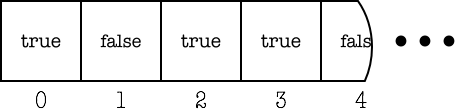
\includegraphics[width=0.5\textwidth]{./img/oracle}
  \caption{Simpele voorstelling van een orakel (bitmap).}
\end{figure}
\vspace{3mm}

Een orakel kan voor vele problemen gebruikt worden. Het halting probleem is hier echter maar \'e\'en enkel voorbeeld van. Vaak wordt een orakel gebruikt om op een abstracte manier een antwoord te krijgen op een bepaalde vraag. Deze vraag kan zelfs onoplosbaar zijn.

\subsubsection*{Krachtiger dan een Turingmachine}

Zoals zonet vermeld, is een orakelmachine krachtiger dan een Turingmachine. Dit wil zeggen dat een orakelmachine sowiso meer talen kan beslissen dan een Turingmachine. Het kan namelijk alle talen beslissen die een Turingmachine kent vermeerderd met heel wat talen die anders in een oneindige lus zullen komen. $A_{TM}$ is daar een voorbeeld van. Een orakelmachine is dus strikt krachtiger dan een Turingmachine.

\subsubsection*{Verzameling orakelmachines}

Normaal wordt een orakelmachine gegeven en kunnen we deze vraag concreet beantwoorden. Dit is nu dus onmogelijk. De redenering gaat echter van de volgende vorm zijn.
\\\\
Een orakel $O^A$ is gegeven dat een taal $A$ beslist. Volgens de definitie van Turingreduceerbaar (zie onderaan) kunnen we concluderen dat elke $B$, waarvoor geldt dat $B \leq_T A$, kan beslist worden door de orakelmachine $O^B$. Het is dus niet mogelijk om alle talen te beslissen, enkel die die Turingreduceerbaar zijn.

\begin{theorem}[Turingreduceerbaar]
	Een taal $A$ is Turingreduceerbaar naar taal $B$, indien $A$ beslisbaar is relatief t.o.v. $B$, t.t.z. er bestaat een orakelachine $O^B$ die $A$ beslist. De notatie is $A \leq_T B$.
\end{theorem}

Het is misschien wel mogelijk om een orakel te ontwerpen dat dit wel kan. In plaats van een bitmap voor alle strings, maken we een bitmap voor alle talen. Een element bevat hier geen booleaanse waarde, maar een ander orakel voor de overeenkomstige taal. Theoretisch is dit volgens mij mogelijk, maar gaat misschien iets te ver voor op het examen.

\subsubsection*{Beslisbaarheid $A_{TM}$ en $H_{TM}$}

Dit is een bijvraag en hier gaan we dus niet dieper op in. De bewijzen van de onbeslisbaarheid worden hier dus niet gegeven. Deze staan ook al in andere vragen. Volgens mij kan hier heel beknopt op geantwoord worden. $A_{TM}$ en $H_{TM}$ zijn niet beslisbaar met standaard Turingmachines. Met een orakelmachine kunnen we uiteraard een corresponderende bitmap maken voor de talen en zijn ze dus wel beslisbaar.